\documentclass{article}

\usepackage{amsmath, amsthm, amssymb, amsfonts}
\usepackage{thmtools}
\usepackage{graphicx}
\usepackage{setspace}
\usepackage{geometry}
\usepackage{float}
\usepackage{hyperref}
\usepackage[utf8]{inputenc}
\usepackage[english]{babel}
\usepackage{framed}
\usepackage[dvipsnames]{xcolor}
\usepackage{tcolorbox}

\newcommand{\HRule}[1]{\rule{\linewidth}{#1}}

\newcommand{\dsanote}[1]{\textbf{[dsa: #1]}}

% ------------------------------------------------------------------------------

\begin{document}

% ------------------------------------------------------------------------------
% Cover Page and ToC
% ------------------------------------------------------------------------------

\title{ \normalsize \textsc{}
		\\ [2.0cm]
		\HRule{1.5pt} \\
		\LARGE \textbf{Parallel and Distributed Computing
		\HRule{2.0pt} \\ [0.6cm] \LARGE{Project Report - MPI Delivery} \vspace*{10\baselineskip}}
		}
\date{}
\author{\textbf{Authors} \\ 
		Carolina Coelho - 99189\\
		Diogo Melita - 99202\\
		Diogo Antunes - 99210}
\maketitle
\newpage

% ------------------------------------------------------------------------------

\section{Introduction}
The goal for this stage is to parallelize the first version fo the \texttt{lifed3d} 
program using MPI.

\section{1st Approach}

In the \texttt{OpenMP} phase, it was already established which part of the code needed parallelization. 
The main challenge then shifted to parallelizing the computation of successive generations across 
different machines and consolidating the results onto a single machine.

\subsection{Data Decomposition}

The initial and arguably crucial step in this stage involved determining how the grid would be 
divided among the various machines. The primary functional approach devised was to partition the 
grid into multiple horizontal slices, with each slice allocated to a different machine. It's 
worth noting that these slices were partitioned to ensure that each had a similar size, thus 
maintaining load balance across the various machines during computation.

This approach led to the decision that each machine would only need to allocate resources for the 
slice it was assigned, effectively reducing the program's memory usage on each machine. Following 
the grid partitioning, the next crucial step was determining how communication between the machines 
would be managed. Given the horizontal partitioning of the grid, each machine would only need to 
communicate with the adjacent machines—specifically, the previous and next machines. During this 
communication, the involved machines would exchange their borders, as these are necessary for 
computing the next generation of border cells.


As each machine only allocates resources for the slice it was assigned to and communicates solely 
with the previous and next machines, it follows that each machine will allocate an additional 
$2 \times n \times n$ cells for the borders of the neighboring slices.

\subsection{Next generation computation}

Once the grid is generated and partitioned among the different machines, the subsequent step is to compute 
the next generations of the grid and assess its status. The core of this code segment closely resembles 
that of previous stages, with the distinction that each machine only computes the next generation 
of the slice it was assigned to. Furthermore, akin to previous stages, the initial statistics of the grid 
are computed before determining the next generations, albeit with the aforementioned difference.

It is crucial to note that since different machines, each with its own memory, are utilized in this stage, 
the computed statistics are only local to each machine. Consequently, these statistics need to be 
consolidated into a single entity, specifically the master machine.

\subsection{Communication}
As previously mentioned, the initial step in transitioning to the simulation phase is to compute the initial 
statistics of the grid. Given that each machine computes only its local statistics, it becomes necessary to 
consolidate the statistics of each machine into a single machine. To achieve this, the \texttt{MPI\_Ireduce} function
was employed. This function was selected for its non-blocking nature, allowing work to continue while communication 
takes place until the results are required.

In this stage, since each machine already possesses the initial neighboring cells of its borders at the outset, it 
can initially compute the next generation of its slice and subsequently update the borders. As a result, the requested 
reduction results are only needed after border exchanges. Therefore, the \texttt{MPI\_Wait} function is utilized to wait 
for the completion of the reduction process.


Border exchanging is facilitated through the use of the \texttt{MPI\_Isend} and \texttt{MPI\_Irecv} functions.
These functions were chosen for their non-blocking nature, allowing work to proceed while communication is underway. 
In this context, the intermediate work entails updating the grid status by the master machine. Subsequently, the 
\texttt{MPI\_Waitall} function is employed to await the completion of the border exchange process.

When using the \texttt{MPI\_Isend} and \texttt{MPI\_Irecv} methods, could have be used the communication time to 
perform the computation of grid values that did not require accessing the border values. However, after conducting 
several measurements of communication time, it was concluded that it is negligible and does not 
justify the aforementioned approach.

Following this, it becomes necessary to reduce the statistics computed at the beginning of the simulation. 
This is accomplished using the \texttt{MPI\_Ireduce} function, as previously mentioned, given that the results 
are required only after the border exchange has been completed.

It's crucial to highlight that due to the utilization of the \texttt{MPI\_Ireduce} function, each machine must uphold 
two arrays for the statistics, exchanged before each generation, akin to the grids. This precaution is necessary to 
prevent potential corruption of statistics, attributable to the non-blocking nature of the function, which permits concurrent 
work while communication is in progress.

%Horizontal slicing
%Two dimensions
%Cubes

%Argue that $n >> p$, so we can just give $n**2$ blocks. Also makes it simpler
%to reason about what information must be exchanged

\dsanote{Try with different data decomposition}

\section{??}

\dsanote{Make a plot with the efficiency}
\dsanote{Maybe recall amdal law and check whether it applies}
\dsanote{Gustafson's law}
\dsanote{Measure load balance in machines}

\dsanote{The impact of latency is speedup} -> use experiments with \texttt{-N}

% ist199202@borg:/mnt/cirrus/users/0/2/ist199202/dsa/src/mpi$ srun -n 64 ./life3d-mpi 3 1024 .4 100
% Took: 2.7s
% Communication time: 0.0s
% Reduce time: 0.1s
% Computation time: 2.5s
% 1 99923786 1
% 2 90413714 1
% 3 83137654 1
% 4 77287897 1
% 5 72448825 1
% 6 68444736 1
% 7 65198270 1
% 8 62633412 1
% 9 60611199 1
% ist199202@borg:/mnt/cirrus/users/0/2/ist199202/dsa/src/mpi$ srun -N 64 ./life3d-mpi 3 1024 .4 100
% Took: 8.6s
% Communication time: 0.1s
% Reduce time: 6.2s
% Computation time: 2.4s
% 1 99923786 1
% 2 90413714 1
% 3 83137654 1
% 4 77287897 1
% 5 72448825 1
% 6 68444736 1
% 7 65198270 1
% 8 62633412 1
% 9 60611199 1

% Add MPI_Barrier and one can conclude that it's because some nodes block waiting for others

\section{Hybrid approach}

Say that the cluster is actually more of a NUMA, so a hybrid approach seems
to be a better fit than a UMA architecture.

Section text

\section{Results}

\begin{table}[h!]
	\centering
	\begin{tabular}{||c c c c c c||} 
	 \hline
	 Version & Number of Nodes & Input 1 & Input 2 & Input 3 & Input 4\\ [0.5ex] 
	 \hline\hline
	 serial & $N/A$ & 13.2 & 20.8 & 72.5 & 168.1 \\ 
	 mpi & 8 & 1.8 & 2.3 & 7.2 & 16.9 \\ 
	 mpi & 16 & 0.9 & 1.2 & 3.9 & 8.5  \\
	 mpi & 32 & 0.7 & 0.9 & 2.9 & 6.8 \\
	 mpi & 64 & 0.4 & 0.5 & 1.5 & 3.7 \\ [1ex] 
	 \hline
	\end{tabular}
	\caption{Times of execution, in seconds, of the serial and parallelized versions of the code.}
	\label{execution-times}
\end{table}

\begin{table}[h!]
	\centering
	\begin{tabular}{||c c c c c c||} 
	 \hline
	 Version & Number of Nodes & Input 1 & Input 2 & Input 3 & Input 4\\ [0.5ex] 
	 \hline\hline
	 mpi & 8 & 7.3 & 9 & 10.1 & 9.9 \\ 
	 mpi & 16 & 14.7 & 17.3 & 18.6 & 19.8  \\
	 mpi & 32 & 18.9 & 23.1 & 25 & 24.7 \\
	 mpi & 64 & 33 & 41.6 & 48.6 & 45.4 \\ [1ex] 
	 \hline
	\end{tabular}
	\caption{Speedup achieved with the parallelized versions of the code, comparing to the serial version}
	\label{speedup}
\end{table}

\begin{figure}[htbp]
    \centering
    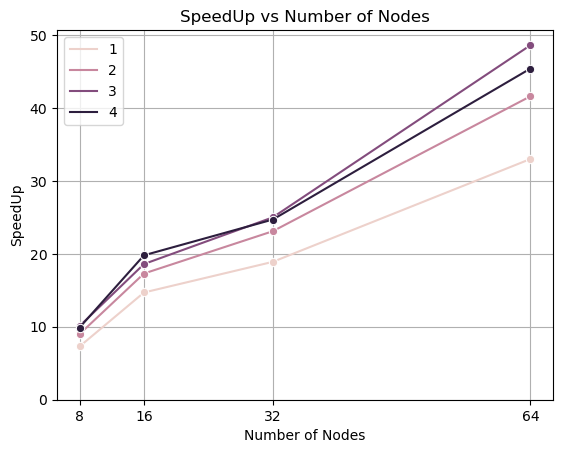
\includegraphics[width=0.5\textwidth]{img/speedup.png}
    \caption{Speedup achieved by the parallelized version when running on different number of nodes.}
    \label{speedup-graph}
\end{figure}

\begin{table}[h!]
	\centering
	\begin{tabular}{||c c c c c c c||} 
	 \hline
	 Version & Number of Nodes & Number of Threads & Input 1 & Input 2 & Input 3 & Input 4\\ [0.5ex] 
	 \hline\hline
	 mpi-omp & 16 & 4 & 0.5 & 0.6 & 1.7 & 3.8 \\  [1ex] 
	 \hline
	\end{tabular}
	\caption{Times of execution, in seconds, of the mpi + omp version of the code.}
	\label{times-mpi-omp}
\end{table}


\newpage

% ------------------------------------------------------------------------------
% Reference and Cited Works
% ------------------------------------------------------------------------------

\bibliographystyle{IEEEtran}
% \bibliography{References.bib}

% ------------------------------------------------------------------------------

\end{document}
